\appendix

\chapter{Matrices Analysis}
\section{The Gradient Field}
\begin{itemize}
    \item For a scalar function of three independent variables $f(x_{1},x_{2},x_{3})$ the gradient is given by the vector equation
    \begin{equation}
        \begin{split}
            \nabla f = \frac{\partial f}{\partial x_{1}}{\hat {x}}_{1} + \frac{\partial f}{\partial x_{2}}{\hat {x}}_{2} + \frac{\partial f}{\partial x_{3}}{\hat {x}}_{3}\\
        \end{split}
    \end{equation}
    \item This can be seen as the derivative of a scalar with respect to a vector, and its result can be easily collected in vector form
    \begin{equation}
        \nabla f = \frac{\partial f}{\partial\mathbf{x}} = 
        \left(
        \begin{array}{c}
            \frac{\partial f}{\partial x_{1}} \\ 
            \frac{\partial f}{\partial x_{2}} \\ 
            \frac{\partial f}{\partial x_{3}}
        \end{array}
        \right)
    \end{equation}
\end{itemize}            


\section{Inner Products}
Let's proof the inner product of vectors.
\begin{figure}[!htbp]
    \centering
    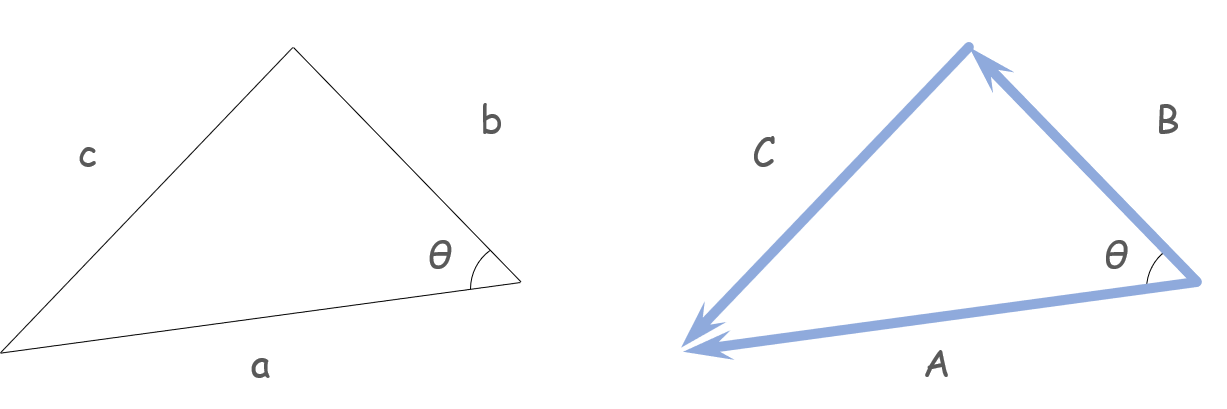
\includegraphics[width=3.6in]{./images/The law of cosine and the angle between vectors.png}
    \caption{The law of cosine and the angle between vectors}
\end{figure}
Recall the law of cosines
\begin{equation} a^2 + b^2 - 2ab\cos\theta = c^2\end{equation}
Apply this to vector triangle
\begin{equation} \left\| \mathbf{A} \right\|^2 + \left\| \mathbf{B} \right\|^2 - 2\left\| \mathbf{A} \right\|\left\| \mathbf{B} \right\|\cos\theta = \left\| \mathbf{A} - \mathbf{B} \right\|^2\end{equation}
Where
\begin{equation} 
    \begin{aligned}
        \left\| \mathbf{A} - \mathbf{B} \right\|^2 &= \left(\mathbf{A}-\mathbf{B}\right) \cdot \left(\mathbf{A}-\mathbf{B}\right) \\
                                                   &= \left\| \mathbf{A} \right\|^2 + \left\| \mathbf{B} \right\|^2 -2\mathbf{A}\cdot\mathbf{B}\\
    \end{aligned}
\end{equation}
This gives
\begin{equation}
    \cos\theta = \frac{\mathbf{A}\cdot\mathbf{B}}{\left\|\mathbf{A}\right\|\left\|\mathbf{B}\right\|}
\end{equation}


\section{Eigenvalues And Eigenvectors}
\begin{itemize}
    \item For a scalar function of three independent variables $f(x_{1},x_{2},x_{3})$ the gradient is given by the vector equation
\end{itemize}            


\section{Singular Value Decomposition}
\begin{itemize}
    \item For a scalar function of three independent variables $f(x_{1},x_{2},x_{3})$ the gradient is given by the vector equation
\end{itemize}            




\chapter{Cheat sheet}
\section{Linear Regression vs Logistic Regression}
\begin{table}[H]
    \renewcommand\arraystretch{1.5}
    \caption{Linear Regression vs Logistic Regression (w/ regularizer)}
    \centering
    \begin{tabular}[t]{lll}     
        \hline 
        \hline 
        Items            & Linear Regression             & Logistic Regression       \\ 
        \hline 
        \hline 
        Cost             & \multirow{2}{*}{$\begin{array}{l} J\left(\theta\right) = \frac{1}{2m} \sum_{i=1}^{m} \left( \mathbf{x}^{(i)}\theta - y^{(i)} \right)^2 \end{array}$}                            & \multirow{2}{*}{$\begin{array}{l} J(\theta) = -\frac{1}{m} \sum_{i=1}^{m} \left[ {y^{(i)}\log{(h^{(i)})}+(1-y^{(i)})\log{(1-h^{(i)})}} \right] \end{array}$} \\
        (original)       &                                                                                                                                                                                 &                                                                                                                                                              \\
        \hline 
        Cost             & \multirow{2}{*}{$\begin{array}{l} J\left(\theta\right) = \frac{1}{2m} \left( \mathbf{X}\theta - \mathbf{y} \right)^T \left( \mathbf{X}\theta - \mathbf{y} \right) \end{array}$} & \multirow{2}{*}{$\begin{array}{l} J(\theta) = -\frac{1}{m} \left( \mathbf{y}^T\log{(\mathbf{h})} + \mathbf{(1-y)}^T\log{(\mathbf{1-h})} \right) \end{array}$}\\ 
        (vectorized)     &                                                                                                                                                                                 &                                                                                                                                                              \\ 
        \hline 
        Gradient descent & \multirow{2}{*}{$\begin{array}{l} \theta_j \coloneqq \theta_j - \frac{\alpha}{m} \sum_{i=1}^{m}\left( h^{(i)} - y^{(i)} \right) x_j^{(i)} \end{array}$}                         & \multirow{2}{*}{Same as linear regression}                                                                                                                   \\
        (original)       &                                                                                                                                                                                 &                                                                                                                                                              \\
        \hline 
        Gradient descent & \multirow{2}{*}{$\begin{array}{l} \theta  \coloneqq \theta - \frac{\alpha}{m}\mathbf{X}^T\left(\mathbf{X}\theta-\mathbf{y}\right) \end{array}$}                                 & \multirow{2}{*}{Same as linear regression}                                                                                                                   \\
        (vectorized)     &                                                                                                                                                                                 &                                                                                                                                                              \\ 
        \hline 
        Normal equation  & $\begin{array}{l} \theta = \left(\mathbf{X}^T\mathbf{X}\right)^{-1}\mathbf{X}^T\mathbf{y} \end{array}$                                                                          & None                                                                                                                                                         \\ 
        \hline
        \hline
    \end{tabular}
\end{table}